\documentclass[a4paper,12pt]{article}
%%%%%%%%%%%%%%%%%%%%%%%%%%%%%%%%%%%%%%%%%%%%%%%%%%%%%%%%%%%%%%%%%%%%%%%%%%%%%%%%%%%%%%%%%%%%%%%%%%%%%%%%%%%%%%%%%%%%%%%%%%%%%%%%%%%%%%%%%%%%%%%%%%%%%%%%%%%%%%%%%%%%%%%%%%%%%%%%%%%%%%%%%%%%%%%%%%%%%%%%%%%%%%%%%%%%%%%%%%%%%%%%%%%%%%%%%%%%%%%%%%%%%%%%%%%%
\usepackage{eurosym}
\usepackage{vmargin}
\usepackage{amsmath}
\usepackage{graphics}
\usepackage{epsfig}
\usepackage{subfigure}
\usepackage{fancyhdr}
%\usepackage{listings}
\usepackage{framed}
\usepackage{graphicx}

\setcounter{MaxMatrixCols}{10}
%TCIDATA{OutputFilter=LATEX.DLL}
%TCIDATA{Version=5.00.0.2570}
%TCIDATA{<META NAME="SaveForMode" CONTENT="1">}
%TCIDATA{LastRevised=Wednesday, February 23, 2011 13:24:34}
%TCIDATA{<META NAME="GraphicsSave" CONTENT="32">}
%TCIDATA{Language=American English}

\pagestyle{fancy}
\setmarginsrb{20mm}{0mm}{20mm}{25mm}{12mm}{11mm}{0mm}{11mm}
\lhead{Graphical Techniques} \rhead{Kevin O'Brien}
\chead{Statistical Quality Control}


\begin{document}
\tableofcontents
\newpage
\section{Cause and Effect Diagrams}

\begin{framed}
\begin{verbatim}
cause.and.effect(cause=list(
  Measurements=c("Micrometers", "Microscopes", "Inspectors"),
  Materials=c("Alloys", "Lubricants", "Suppliers"),
  Personnel=c("Shofts", "Supervisors", "Training", "Operators"),
  Environment=c("Condensation", "Moisture"),
  Methods=c("Brake", "Engager", "Angle"),
  Machines=c("Speed", "Lathes", "Bits", "Sockets")),
effect="Surface Flaws")
\end{verbatim}
\end{framed}
\begin{figure}[h!]
\centering
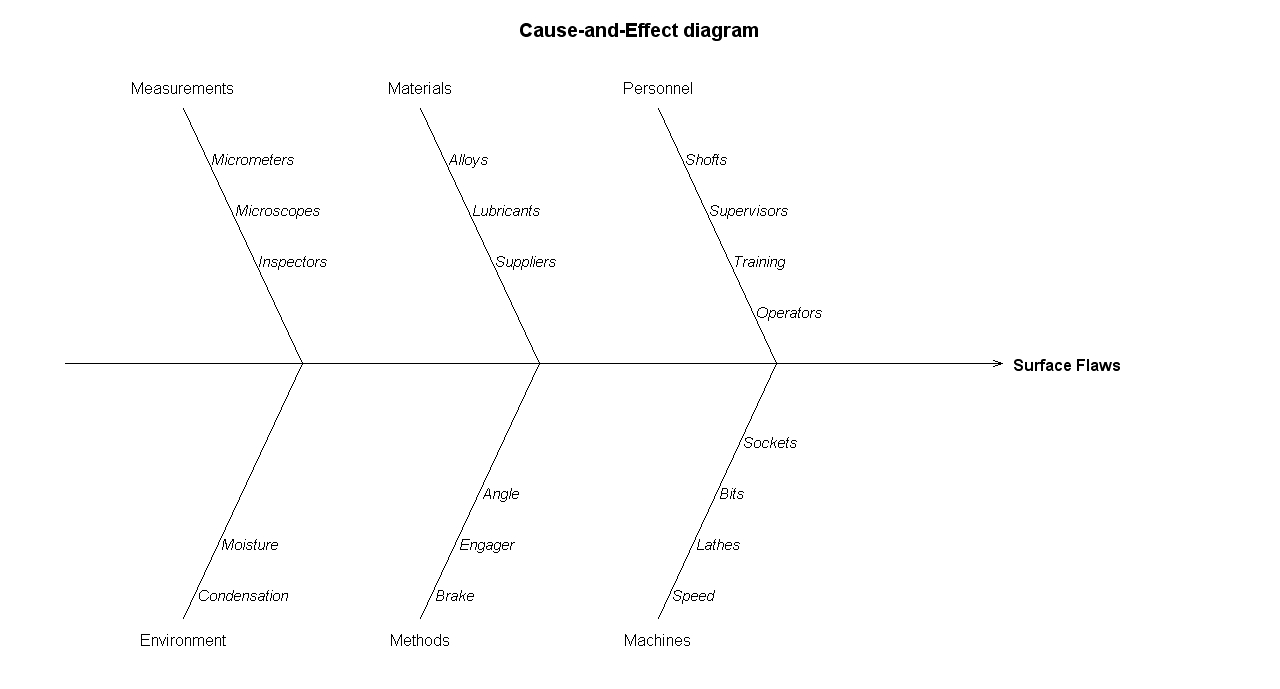
\includegraphics[width=0.7\linewidth]{./qccfishbone}
\caption{}
\label{fig:qccfishbone}
\end{figure}

\newpage
\section{Pareto Chart Analysis.}
 Quality problems are rarely spread evenly across the different aspects of the production process or different plants. Rather, a few "bad apples" often account for the majority of problems. This principle has come to be known as the Pareto principle, which basically states that quality losses are mal-distributed in such a way that a small percentage of possible causes are responsible for the majority of the quality problems. For example, a relatively small number of "dirty" cars are probably responsible for the majority of air pollution; the majority of losses in most companies result from the failure of only one or two products. To illustrate the "bad apples", one plots the Pareto chart,
\newpage
\section{Pareto Analysis (Implementation with qcc package)}
\begin{framed}
\begin{verbatim}
defect <- c(80, 27, 66, 94, 33)

names(defect) <- c("price code", "schedule date", 
 "supplier code", "contact num.", "part num.")

# 1
pareto.chart(defect, ylab = "Error frequency")

#2
pareto.chart(defect, ylab = "Error frequency", xlab = "Error causes", las=1)

#3
pareto.chart(defect, ylab = "Error frequency", col=rainbow(length(defect)))

#4
pareto.chart(defect, cumperc = seq(0, 100, by = 5), 
    ylab2 = "A finer tickmarks grid")

\end{verbatim}
\end{framed}
\textbf{Output to accompany graphs}
\begin{verbatim}
Pareto chart analysis for defect
                Frequency Cum.Freq. Percentage Cum.Percent.
  contact num.         94        94   31.33333     31.33333
  price code           80       174   26.66667     58.00000
  supplier code        66       240   22.00000     80.00000
  part num.            33       273   11.00000     91.00000
  schedule date        27       300    9.00000    100.00000
\end{verbatim}
%------------------------------------------- %
\newpage

\begin{figure}[h!]
\centering
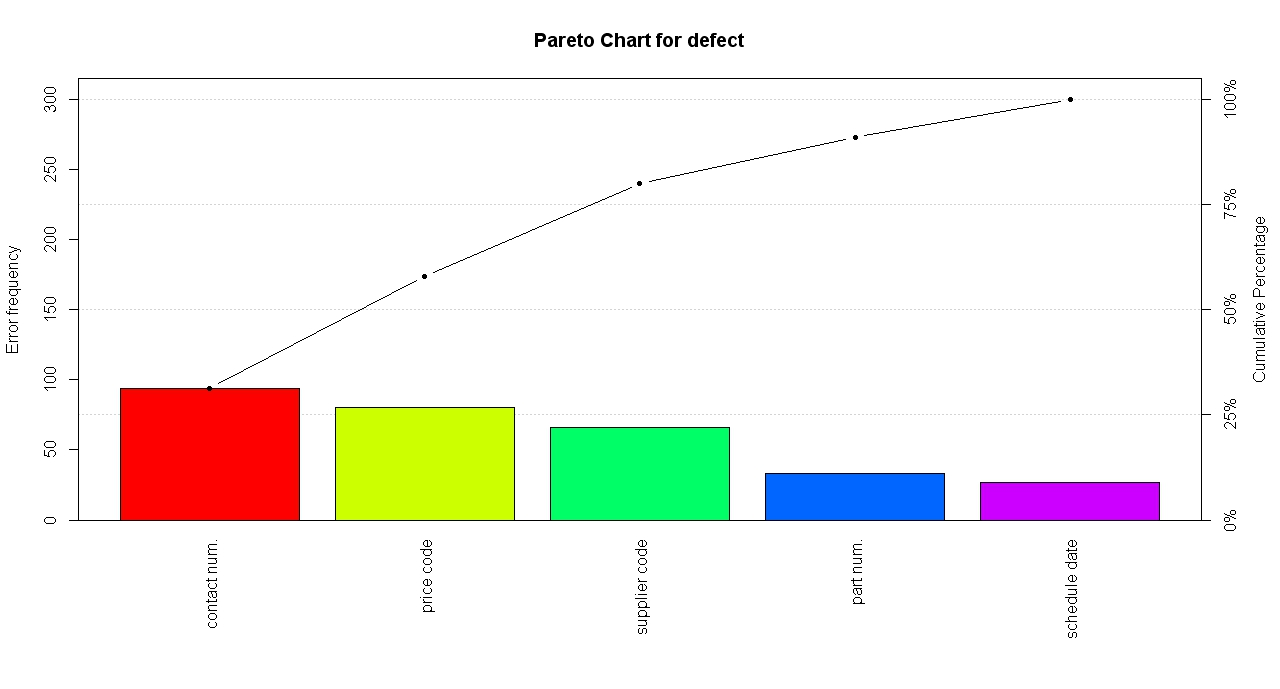
\includegraphics[width=0.8\linewidth]{./Pareto3}
\caption{Third Implementation}
\label{fig:Pareto3}
\end{figure}

\begin{figure}[h!]
\centering
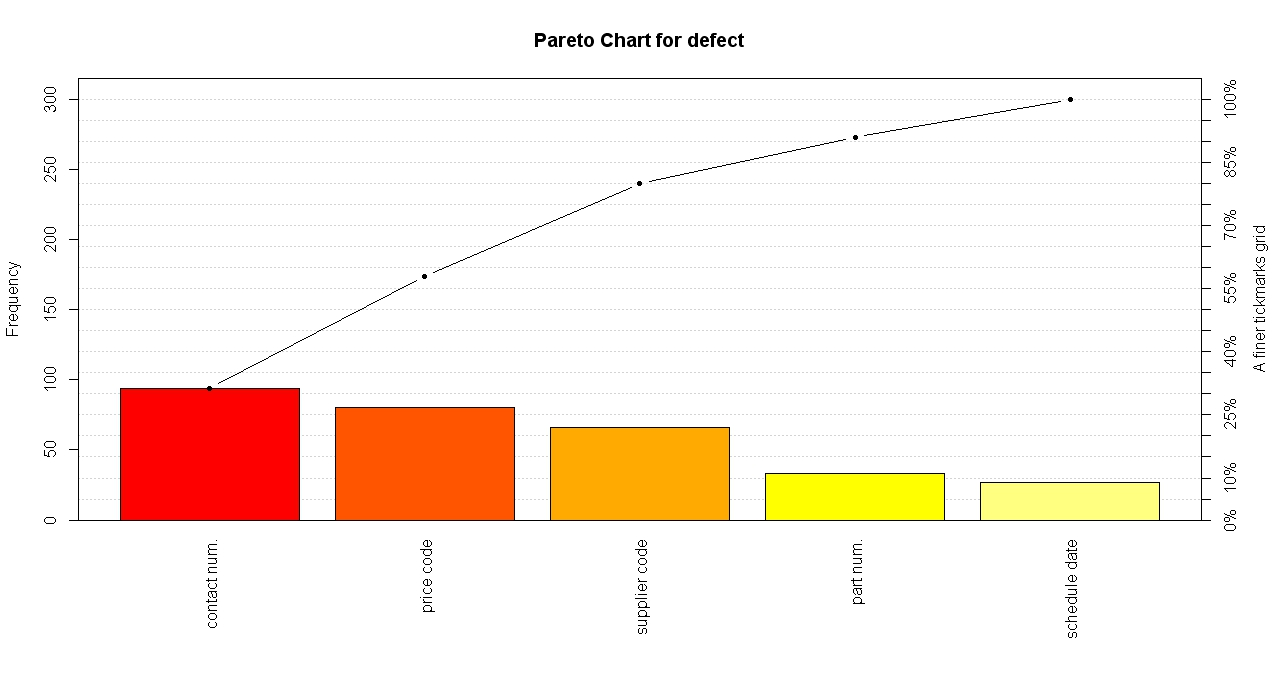
\includegraphics[width=0.8\linewidth]{./Pareto5}
\caption{Fourth Implementation}
\label{fig:Pareto5}
\end{figure}
%------------------------------------------- %


\newpage
\section{Operating Characteristic (OC) Curves}
\begin{itemize}
\item A common supplementary plot to standard quality control charts is the so-called operating characteristic or OC curve (see example below). One question that comes to mind when using standard variable or attribute charts is how sensitive is the current quality control procedure? Put in more specific terms, how likely is it that you will not find a sample (e.g., mean in an X-bar chart) outside the control limits (i.e., accept the production process as "in control"), when, in fact, it has shifted by a certain amount? 

\item This probability is usually referred to as the  (beta) error probability, that is, the probability of erroneously accepting a process (mean, mean proportion, mean rate defectives, etc.) as being "in control." 

\item Note that operating characteristic curves pertain to the false-acceptance probability using the sample-outside-of- control-limits criterion only, and not the runs tests described earlier.


\item Operating characteristic curves are extremely useful for exploring the power of our quality control procedure. The actual decision concerning sample sizes should depend not only on the cost of implementing the plan (e.g., cost per item sampled), but also on the costs resulting from not detecting quality problems. The OC curve allows the engineer to estimate the probabilities of not detecting shifts of certain sizes in the production quality.
\end{itemize}






\newpage
\subsection{pistonrings Data}
\begin{framed}
\begin{verbatim}
data(pistonrings); attach(pistonrings);

diameter <- qcc.groups(diameter, sample)
beta <- oc.curves.xbar(qcc(diameter, type="xbar", nsigmas=3, plot=FALSE))
print(round(beta, digits=4))

# or to identify points on the plot use
## Not run: oc.curves.xbar(qcc(diameter, 
    type="xbar", nsigmas=3, plot=FALSE), identify=TRUE)

detach(pistonrings)
\end{verbatim}
\end{framed}


\newpage
\subsection{orangejuice Data}
\begin{framed}
\begin{verbatim}
data(orangejuice)
attach(orangejuice)
beta <- oc.curves(qcc(D[trial], sizes=size[trial], type="p", plot=FALSE))
print(round(beta, digits=4))
# or to identify points on the plot use
## Not run: oc.curves(qcc(D[trial], sizes=size[trial], type="p", plot=FALSE), identify=TRUE)
detach(orangejuice)
\end{verbatim}
\end{framed}
\newpage
\subsection{circuit Data}
\begin{framed}
\begin{verbatim}
data(circuit)
attach(circuit)
q <- qcc(x[trial], sizes=size[trial], type="c", plot=FALSE)
beta <- oc.curves(q)
print(round(beta, digits=4))
# or to identify points on the plot use
## Not run: oc.curves(qcc(x[trial], sizes=size[trial], type="c", plot=FALSE), identify=TRUE)
detach(circuit)
\end{verbatim}
\end{framed}
\newpage
\section{Moving Average (MA) Chart}
To return to the piston ring example, suppose we are mostly interested in detecting small trends across successive sample means. For example, we may be particularly concerned about machine wear, leading to a slow but constant deterioration of quality (i.e., deviation from specification). The CUSUM chart described above is one way to monitor such trends, and to detect small permanent shifts in the process average. 

Another way is to use some weighting scheme that summarizes the means of several successive samples; moving such a weighted mean across the samples will produce a moving average chart (as shown in the following graph).



\section{Exponentially-weighted MA (EWMA) Chart}
The idea of moving averages of successive (adjacent) samples can be generalized. In principle, in order to detect a trend we need to weight successive samples to form a moving average; however, instead of a simple arithmetic moving average, we could compute a geometric moving average (this chart (see graph below) is also called Geometric Moving Average chart, see Montgomery, 1985, 1991).
%-------------------------------------------------- %
\newpage
\subsubsection{Grouped Data}
\begin{framed}
\begin{verbatim}

data(pistonrings)
attach(pistonrings)
diameter <- qcc.groups(diameter, sample)
q <- ewma(diameter[1:25,], lambda=0.2, nsigmas=3)
summary(q)

q <- ewma(diameter[1:25,], lambda=0.2, nsigmas=2.7,
newdata=diameter[26:40,], plot = FALSE)
summary(q)

plot(q)
\end{verbatim}
\end{framed}

\begin{figure}[h!]
\centering
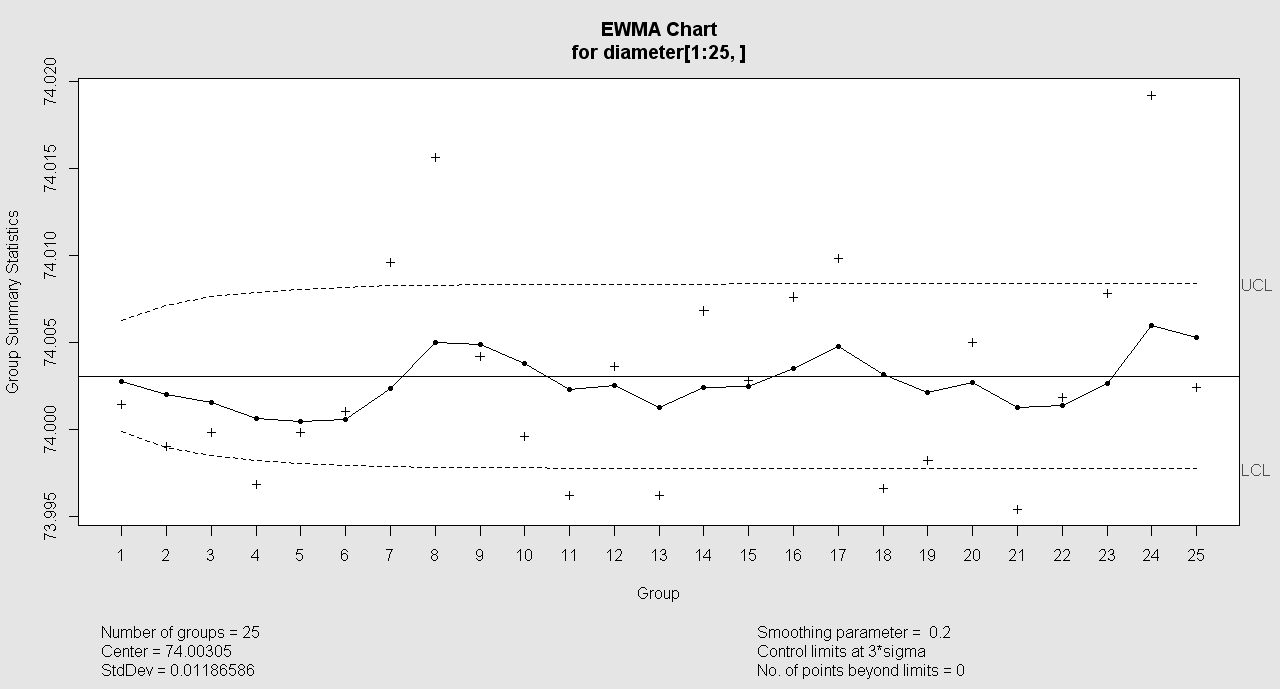
\includegraphics[width=0.6\linewidth]{./qccEWMA1}
\caption{}
\label{fig:qccEWMA1}
\end{figure}
\begin{figure}[h!]
\centering
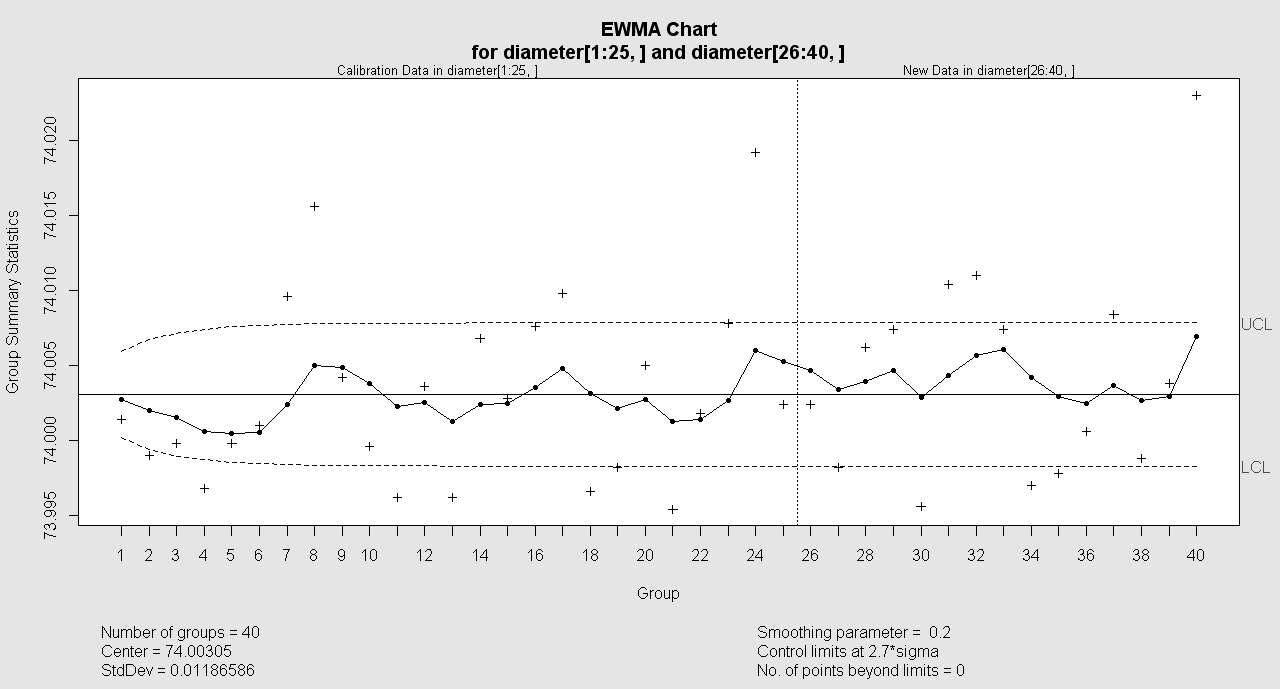
\includegraphics[width=0.6\linewidth]{./qccEWMA2}
\caption{}
\label{fig:qccEWMA2}
\end{figure}
\begin{verbatim}
> summary(q)

Call:
ewma(data = diameter[1:25, ], lambda = 0.2, nsigmas = 2.7, newdata = diameter[26:40,     ], plot = FALSE)

ewma chart for diameter[1:25, ] 

Summary of group statistics:
   Min. 1st Qu.  Median    Mean 3rd Qu.    Max. 
  74.00   74.00   74.00   74.00   74.01   74.02 

Group sample size:  5
Number of groups:  25
Center of group statistics:  74.00305
Standard deviation:  0.01186586 

Summary of group statistics in diameter[26:40, ]:
   Min. 1st Qu.  Median    Mean 3rd Qu.    Max. 
  74.00   74.00   74.00   74.00   74.01   74.02 

Group sample size:  5
Number of groups:  15 

Smoothing parameter: 0.2 
Control limits:
         LCL      UCL
1   74.00018 74.00591
2   73.99938 74.00672
...                  
40  73.99827 74.00782

\end{verbatim}
\newpage
\subsubsection{Individual observations}
\begin{framed}
\begin{verbatim}
x <- c(33.75, 33.05, 34, 33.81, 33.46, 34.02, 33.68, 33.27, 33.49, 33.20,
33.62, 33.00, 33.54, 33.12, 33.84) # viscosity data (Montgomery, pag. 242)
q <- ewma(x, lambda=0.2, nsigmas=2.7)
summary(q)
\end{verbatim}
\end{framed}

\begin{framed}
\begin{verbatim}
x <- 1:50
y <- rnorm(50, sin(x/5), 0.5)
plot(x,y,pch=16,col="blue",font.lab=2)
lines(ewmaSmooth(x,y,lambda=0.1), col="red")
abline(h=mean(y),col="green",lty=2)
title("EWMA Smoother")
\end{verbatim}
\end{framed}
\begin{figure}
\centering
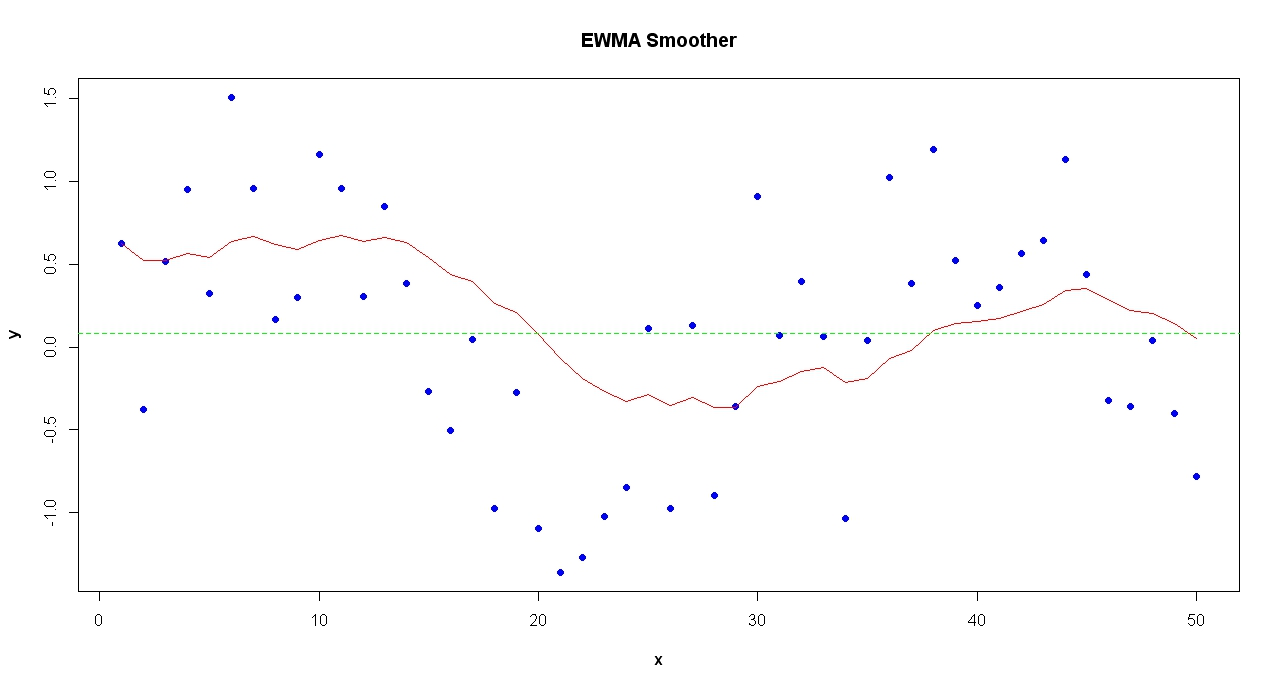
\includegraphics[width=0.7\linewidth]{./qccEWMAsmoother}
\caption{}
\label{fig:qccEWMAsmoother}
\end{figure}

\end{document}